%!TEX root = ../thesis.tex
%*******************************************************************************
%*********************************** First Chapter *****************************
%*******************************************************************************
\chapter{Introduction}  %Title of the First Chapter

\ifpdf
    \graphicspath{{Chapter1/Figs/Raster/}{Chapter1/Figs/PDF/}{Chapter1/Figs/}}
\else
    \graphicspath{{Chapter1/Figs/Vector/}{Chapter1/Figs/}}
\fi


%********************************** %First Section  **************************************
\section{Background and related works} %Section - 1.1 

The demand for Warehouse-Scale Computer (WSC) is on a fast-growing trend, with a different 
architecture and load compared to PC, mobile devices and servers. However, to our knowledge, the 
prediction accuracy of existing predictors under this new type of load has not been explored. This 
project investigates the directional branch prediction accuracy of existing conditional branch 
predictors under WSC load and to compare the results with the accuracy of the predictors 
under other loads.


\subsection{Origin of branch predictor} % 1.1.1
The importance of a high-accuracy branch predictor comes first and foremost from the pipeline penalty. 
Modern CPUs typically have dozens of pipeline stages, which means that once the prediction is wrong 
and the whole pipeline goes in the wrong direction, the cost of washing the pipeline and starting again 
is huge. IPC can be negatively impacted by each wrong prediction.
\par\hspace*{\fill}\par
Besides, there are some critical technologies that rely on accurate branch prediction. For example, 
branch predictor predict the future instructions and feed those instructions into re-order buffer (ROB). 
Apple A14 (2020) and M1 has 600+ ROB entries\cite{frumusanu_apple_2022}, which is massively larger than typical ~300-entry 
re-order buffer in conventional Intel/AMD/Arm processors. Similarly, re-order window of Intel's
Golden Cove (2021) has a huge increase compared with Sunny Cove (2019) – 512 entries compared to 
352\cite{frumusanu_intel_2021}. The trend of the industry is to increase out-of-order buffer size, the idea behind is trying to increase the chance to get executable instruction from ROB. This put pressure on the CPU front-end: to not 
waste those extra ROB spaces, branch predictor must keep high accuracy prediction to keep the ROB 
occupied by correct instructions. Prefetching technology is another example: the industry is also 
heavily relying on high branch prediction accuracy to remove instruction cache misses\cite{ishii_rebasing_2020}.
\par\hspace*{\fill}\par

There are actually two parts of branch prediction, direction prediction predicting whether the 
conditional branch is taken and target prediction predicts the target address of the jump. This project 
focus on directional prediction because it is simpler and thus a very good starting point for a time-sensitive project. Three important branch direction predictor schemes, gShare\cite{mcfarling_combining_1993} and TAGE\cite{seznec_case_2006} (the scheme used by SOTA branch predictor) and Perceptron Predictor\cite{jimenez_dynamic_2001} are introduced later. 


\subsection{Design of branch direction predictors}
\subsubsection{gShare}
GShare was first proposed by Scott McFarling in 1993. The innovative introduction of the XOR mechanism helps the GShare predictor globally identify different branches and reduce the probability of aliasing. 
\par\hspace*{\fill}\par
Gshare use a pattern history table (PHT) consisting of two-bit saturating counters, indexed by a global history register. The structure leads to an exponential growth of the size of PHT with the length of the global history\cite{jimenez_dynamic_2001}.

\subsubsection{Perceptron Predictor}
The perceptron predictor was first introduced into branch predictor by Daniel A. JimCnez and Calvin Lin in 2001. Pereceptron predictor stores weights of each history direction into perceptron and indexes perceptrons only using hashed PC. The capacity increases when size of each perceptron increases, thus achieving linear growth with the history length. 
\par\hspace*{\fill}\par
The limitations of perceptron predictor are, firstly, that it is only good at predicting linearly separable branches because it uses only a single layer of perceptron, and secondly, that the earliest perceptron predictor only uses global histroy for prediction and ignores other branch features.
\par\hspace*{\fill}\par
It's worth to mention that perceptron is becoming a majority in the newly proposed branch predictor schemes, including SRNN predictor\cite{zhang_dynamic_2020} and BranchNet\cite{zangeneh_branchnet_2020}. 

\begin{figure}[htbp!] 
\centering    
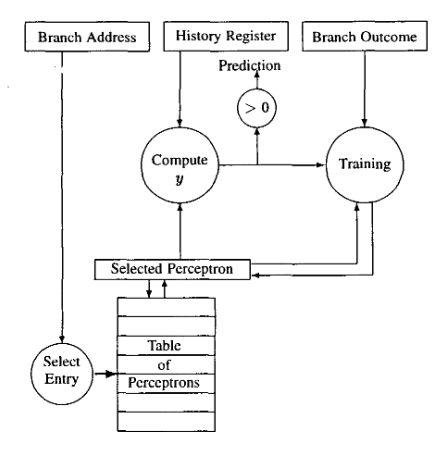
\includegraphics[width=0.5\textwidth]{Chapter1/Figs/perceptron.png}
\caption{\centering Perceptron Predictor Block Diagram\cite{jimenez_dynamic_2001}. }
\label{fig:perceptron2001}
\end{figure} % trace length plot

\newpage
\subsubsection{TAGE}

The history length is a key question for branch predictor. Longer histories enable accurate predictions for some HTP branches while taking more time to warm-up, reducing accuracy for ETP branches. Geometric history length\cite{seznec_analysis_2005} helps find a balance for this question: predictor with shorter history length provides predictions early on before longer predictors finishes warm-up stage. PPM data compression algorithm can be a efficient way to manage and select from predictors with various history length.
\par\hspace*{\fill}\par
TAGE, derived from a PPM-like predictor \cite{michaud_ppm-like_2005} by André Seznec, Pierre Michaud (2006), combines the advantage of geometric history length and PPM data compression algorithm, thus enables more efficient storage of detected patterns.


\subsection{New trends in branch prediction field}

Some new trends and concepts in branch prediction field are briefly mentioned and core reference are cited for future study.

\subsubsection{Security issues}

As the security and privacy of computer systems has become increasingly emphasised, research interest has attracted into the security of branching predictors under side-channel attacks. Side channel attack is based on leaked information from the physical implementation of the cryptosystem rather than theoretical weaknesses in the encryption algorithm. Under this kind of attack, shared directional branch predictor can be manipulated by the attacker and the prediction and  history target can be leaked\cite{evtyushkin_branchscope_2018}. It is difficult for mitigation technique to achieve both performance and isolation, but there are some meaningful attempts\cite{vougioukas_brb_2019}.


\subsubsection{Offline training}

Offline training refers to training of the predictor before the execution of the program and its counterpart is runtime branch prediction. The limited resources on a chip and the low latency requirements limit the scale and complexity of branch prediction algorithms. However, it is possible to improve predictor accuracy by extracting the properties of branch traces in advance for offline training. Offline learning takes place in two main stages: compiling and profiling.

\subsection{Warehouse-scale computer (WSC)} % 1.1.4

In the section, the general idea of WSC is briefly mentioned, followed by emphasising the key features of the WSC that may affect the work of branch predictor. \par\hspace*{\fill}\par

WSCs are a kind of datacenter that provide large-scale, high-performance, low-cost Internet, computing and storage services\cite{barroso_datacenter_2013}. Born out of the demand for large-scale computing for a small amount of applications (e.g. webmail, web search, online translation), in recent years it has gradually taken over a large amount of computing and storage demands that would otherwise have been carried out locally as the price of computing power has fallen. \par\hspace*{\fill}\par

However, WSCs are fundamentally distinct from traditional benchmarks due to the need for on-demand scalability, elasticity and availability. Unlike traditional datacenter where a number of independent and different machines are physically put together, machines in WSC are more homogeneous, emphasising internal connection. Machines often have similar hardware architectures, run on the same software platform, and are connected and managed under the same system management layer. \par\hspace*{\fill}\par

WSCs run a small number of super-scale tasks, usually on thousands of machines simultaneously, flexibly allocating computing power according to demand. Super-scale tasks can have two significant consequences:
\begin{enumerate}[itemsep= 0pt,topsep = 0pt, partopsep=4 pt, leftmargin= 32 pt]
\item Data parallelism arises from large datasets that need to be processed. These large-scale datasets 
often require a large amount of computation for each parallel (sub) task, which may lead to 
periodic, regular instruction streams performed by a single core over a period of time.
\item Executables are also getting bigger. The increased range of instructions makes it harder for 
branch predictors to predict correctly.
In addition, WSC has a greater instruction throughput and typically has a larger reorder window (i.e. 
out-of-order buffer), resulting in a greater reliance on high accuracy branch predictions. However, the 
branch predictor design is not specifically optimised for this critical and unique load.
\end{enumerate}
%********************************** %Second Section  *************************************
\section{Motivations and Objectives} %Section - 1.2

WSC has been in increasing demand and deployment in recent years, and its unique load characteristics are expected to have an impact on branch predictors. Prediction accuracy under such loads has been a gap and is waiting to be investigated. May 2022, google released google datacenter's actual instruction and memory access traces, making research on WSC more feasible and convenient. \par\hspace*{\fill}\par

Here are the main goals of the project. Note that attention is only focused on the directional branch predictors at this stage.\par


\begin{enumerate}[itemsep= 0pt,topsep = 0pt, partopsep=4 pt, leftmargin= 32 pt]
\item (completed) To get familiar with the branch prediction field and compose a well-categorised review of the field, including brief development history, the latest trends and SOTA design.
\item (completed) To setup the required infrastructures on the HUAWEI laptop and server and launch the branch  predictor simulator under default traces. 
\item(completed) To do necessary data processing on Google traces so that it can be accepted by the CBP-5 simulator without losing required information. 
\item(core objective, completed) To evaluate the accuracy of direction prediction vs capacitance of branch predictors (TAGE, perceptron) on Google Workload Traces and compare the results with the prediction accuracy under conventional load.
\end{enumerate}

%********************************** % Third Section  *************************************
\section{Report Organization}  %Section - 1.3 
\label{section1.3}

The report is structured as follows: the second section discusses the method used in the 
simulation. This includes the introduction of simulation infrastructure: CBP-5 simulator kit and Google Workload traces. The method of converting Google WSC traces into CBP-5 BT9 file is also discussed. In the next section, the results of the simulation are presented and discussed in the following order: traces statistic analysis, impact of trace sets on simulation and impact of predictors on simulation results. Some discussion about the conduct on the project is also made in this section. Finally, conclusions are drawn based on the current progress.



